\documentclass[12pt]{beamer}

% Settings & imports
\usetheme[
  numbering=fraction,
  progressbar=frametitle,
]{metropolis}

\usepackage{pgfpages}
\usepackage{movie15}
\setbeameroption{show notes on second screen=right}

% Document config
\title{Blockchain to stimulate local economies}
\date{\today}
\author{Cyril Forveille \and Maxime Lewandowski}
\titlegraphic{\hfill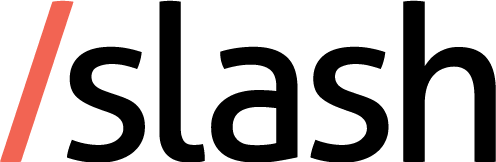
\includegraphics[height=.5cm]{images/slash-logo}}
% \institute{Slash.co}


\begin{document}
  \maketitle



  \section{Complementary currency}

  % Definitions
  \begin{frame}{Local and complementary currency}
    \begin{itemize}
      \item Not a replacement
      \item Different purpose
      \item Solve \alert{local} problems
    \end{itemize}
    \note{Local problems like unemployment, money hoarding}
  \end{frame}

  \begin{frame}{Demurage currency}
    \begin{itemize}
      \item Silivio Gesell
      \item Prevent savings
      \item Increase money velocity
    \end{itemize}
    \note{Money loses value over time}
  \end{frame}

  % Examples
  \begin{frame}{The Wörgl experiment}
    \begin{figure}
      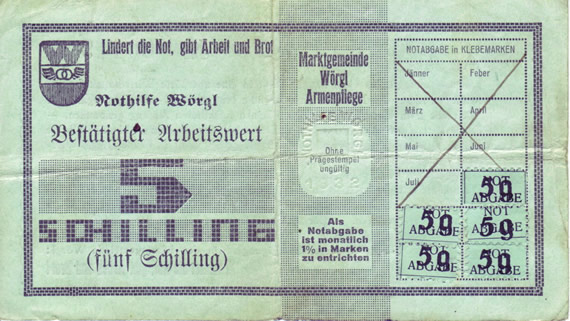
\includegraphics[height=.5\textheight]{images/worgl-5}
      \caption{Wörgl stamp}
    \end{figure}
  \end{frame}

  \begin{frame}{The Wörgl experiment}
    \begin{itemize}
      \item Bills expire after a month
      \item Stamp cost 1\% of bill value
    \end{itemize}
    \note{Austria in 1932}
  \end{frame}

  \begin{frame}{Freicoin}
    \begin{figure}
      
\includegraphics[height=.5\textheight]{images/freicoin}
      \caption{Freicoin logo}
    \end{figure}
  \end{frame}

  \begin{frame}{Freicoin}
    \begin{itemize}
      \item Crypto-currency (PoW based)
      \item $-5$\% a year
      \item Big failure
    \end{itemize}
    \note{Worth nothing nowerdays, susspected to be a scam}
  \end{frame}



  \section{Non-speculative currency}

  % Definition
  \begin{frame}{Non-speculative currency definition}
    \begin{itemize}
      \item \alert{Fixed} exchange rate
      \item \alert{Indexed} on national currency
      \item \alert{Local} \& complementary
    \end{itemize}
  \end{frame}




  \section{Crypto-currency}

  % Definition
  \begin{frame}{Crypto-currency definition}
    \begin{itemize}
      \item Highly \alert{volatile}
      \item Decentralized
      \item Global
    \end{itemize}
    \note{Not backed\\Speculative\\Hackable\\Crime =\} Identity (PoA)}
  \end{frame}




  \section{Our vision}

  \begin{frame}{The vision}
    \begin{itemize}
      \item Boost \alert{local} exchange
      \item Solve \alert{local} unemployment
    \end{itemize}
  \end{frame}

  \begin{frame}{A currency}
    \begin{itemize}
      \item Non-speculative
      \item Demurrage
      \item Local \& complementary
    \end{itemize}
  \end{frame}

  \begin{frame}{A crypto-currency?}
    \begin{itemize}
      \item Free transactions
      \item Decentralized
      \item Demurrage
      \item Free transactions
      \item Local \& complementary
    \end{itemize}
  \end{frame}


  % BREAAAAAAK
  \begin{frame}[standout]
    BREAK
  \end{frame}

  \section{Experience of building decentralized applications}

  % definitions
  \begin{frame}{Decentralization}
    \begin{figure}
      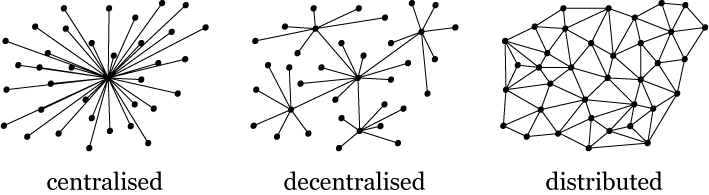
\includegraphics[height=.5\textheight]{images/centralised-decentralised-distributed}
    \end{figure}
  \end{frame}

  \begin{frame}{What is decentralization?}
    \begin{itemize}
      \item Network with \alert{no master}
      \item \alert{Trustless}
      \item No single point of failure
    \end{itemize}
  \end{frame}


  \begin{frame}{How to achieve decentralization?}
    \begin{itemize}
      \item \alert{Smartcontracts}
      \item Custom \alert{consensus} algorithm
    \end{itemize}
  \end{frame}




  \section{Smart contract}

  \begin{frame}{Smart contract}
    \begin{itemize}
      \item \alert{Autonomous} piece of code
      \item Lives on a \alert{blockchain}
      \item \alert{Trackable} activity
      \item \alert{Irreversible} transactions
      \item Many fields of applications
    \end{itemize}
    \note{Voting systems, domain registery, financial exanche, saving account,
    market prediction, crownfounding platform, intellectual property, other
    crypto, \ldots}
  \end{frame}

  \begin{frame}{ERC20}
    \begin{itemize}
      \item Type of \alert{smartcontract}
      \item Lives on the \alert{Ethereum} blockchain
    \end{itemize}
    \begin{itemize}
      \item Safe and Documented
      \item Easy to code and deploy
    \end{itemize}
    \begin{itemize}
      \item Transaction costs money (ether gas)
      \item No control over miners reward
    \end{itemize}
  \end{frame}



  \section{Custom consensus}


  \section{Consensus}

  \begin{frame}{Consensus in blockchain}
    \begin{itemize}
      \item Rules that define the blockchain
      \item Block creation and validation
      \item Many popular consensus
    \end{itemize}
    \note{Major part in blockchain implementation\\
        Rules to take decision on a blockchain, create and validate blocks\\
        Plenty of consensus, we explored the most populars}
  \end{frame}

  \begin{frame}{Proof of work}
    \begin{itemize}
      \item Block creation require CPU usage
      \item Complex mathematical operation
    \end{itemize}
    \note{Used by bitcoin\\
    Solving mathematical problem to hash the new block\\
    Called minning\\
    Reward first miner\\
    Criticized: energy consumption required\\
    Blockchain growing = more amount of energy}
  \end{frame}

  \begin{frame}{Proof of stake}
    \begin{itemize}
      \item Block creation require stake
      \item Use less energy
      \item Has some vulnerabilities
    \end{itemize}
    \note{Same hashing process\\
    Block creator chosen in a deterministic way\\
    Depending on wealth, stake\\
    No block reward\\
    Transaction fee as a reward\\
    Less energy consumption}
  \end{frame}

  \begin{frame}{Delegated proof of stake}
    \begin{itemize}
      \item Proof of stake with voting system
    \end{itemize}
    \note{People vote for the next miner\\
    a few selected peers can work\\
    Vote strength determined by tokens held}
  \end{frame}

  \begin{frame}{Proof of authority}
    \begin{itemize}
      \item Indentity as a stake
      \item Require a central authority
    \end{itemize}
    \note{not anonymous\\
    blocks validated by approved accounts (validators)\\
    identity = reputation\\
    earn the right to become validators\\
    not decentralized}
  \end{frame}

  \begin{frame}{Practical Byzantine fault tolerance}
    \begin{itemize}
      \item State machine replication
      \item Work with malicious nodes
      \item 2/3 votes to reach concensus
    \end{itemize}
    \note{every validator share state\\
    deterministic steps (state machine replication)\\
    work with less 1/3 malicious nodes\\
    }
  \end{frame}

  \begin{frame}{Advantages of PBFT}
    \begin{itemize}
      \item Transaction finality
      \item Energy efficient
      \item Each validator can be rewarded
      \item High performances on small networks
    \end{itemize}
    \note{very effective on small networks (40 nodes)
    }
  \end{frame}

  \section{Our take on those techs}

  \begin{frame}{Build a blockchain from scratch}
    \begin{figure}
      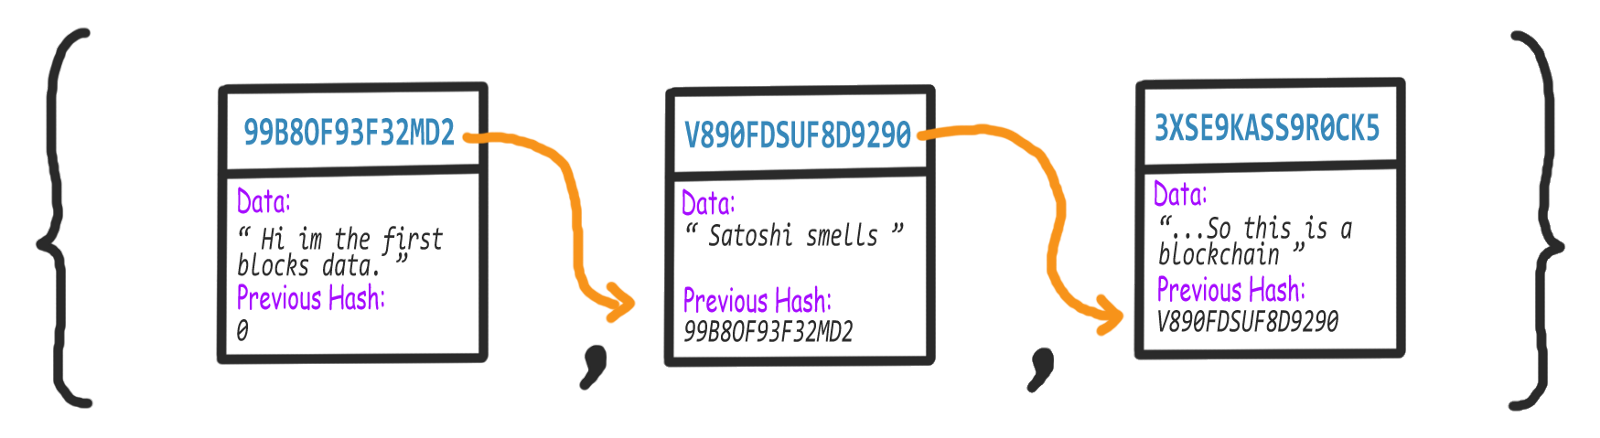
\includegraphics[height=.35\textheight]{images/scratch}
      \caption{blockchain}
    \end{figure}
    \note{more liberties\\choose consensus\\reward miners\\no transaction fees\\do not depend on another blockchain}
  \end{frame}

  \begin{frame}{Istanbul Byzantine fault tolerance (IBFT)}
    \begin{itemize}
      \item Improvement of PBFT
      \item Gossip network
      \item Optimisations
    \end{itemize}
    \note{Implemented by Quorum and a fork of ethereum\\
      Gossip network\\
      More validators with better performances
    }
  \end{frame}

  \begin{frame}{Clique PoA}
    \begin{itemize}
      \item Signers submit blocks
      \item Voting system
      \item Protection against malicious signers
    \end{itemize}
    \note{ signers submit block sequentialy\\
      signers are identified, we can know who submitted\\
      possibility to vote
    }
  \end{frame}

  \begin{frame}{IBFT + PoA}
    \begin{itemize}
      \item Semi-decentralized blockchain
      \item Central authority delivers authorizations
      \item Small network (100 validators)
    \end{itemize}
    \note{semi-decentralized blockchain\\
      central authority (first node) allow validators\\
      fast, secure and low energy consumption
    }
  \end{frame}

  \begin{frame}{Problems encountered}
    \begin{itemize}
      \item Create a TCP communication protocol
      \item A lot of cryptography
      \item Synchronization between validators
    \end{itemize}

  \end{frame}


\end{document}
